 \documentclass[UTF8,12pt]{ctexart}

\usepackage[T1]{fontenc}
\usepackage{newpxtext,newpxmath} % palatino风格字体
\usepackage{geometry} % 调整页边距
\usepackage{algorithm} % 算法伪代码包
\usepackage{algorithmic}
\usepackage[usenames, dvipsnames]{xcolor}
\usepackage{listings} % 代码高亮包
\usepackage{tikz}
\usetikzlibrary{graphs, positioning, quotes, shapes.geometric}
\geometry{a4paper,scale=0.8} % 调整页边距

\ctexset{section={format={\large\bfseries\raggedright}}}  % section居左

\setCJKmainfont[BoldFont=SimHei, ItalicFont=KaiTi]{SimSun} % 字体设置

\newcommand{\BigO}[1]{\ensuremath{\operatorname{O}\bigl(#1\bigr)}}
\newcommand{\BigOmega}[1]{\ensuremath{\operatorname{\Omega}\bigl(#1\bigr)}}

\lstset{
	basicstyle=\ttfamily,% 基本风格
	numberstyle=\ttfamily,
	numbers=left,    % 行号
	numbersep=10pt,  % 行号间隔 
	tabsize=4,       % 缩进
	extendedchars=true, % 扩展符号?
	breaklines=true, % 自动换行
	language=C++,
	showspaces=false,% 空格字符加下划线
	showstringspaces=false,% 字符串中的空格加下划线
	showtabs=false,  % 字符串中的tab加下划线
	breaklines=true,
	frame=shadowbox,
	rulesepcolor=\color{red!20!green!20!blue!20},
	keywordstyle=\color{Fuchsia},       % keyword style
	stringstyle=\color{teal},
	commentstyle=\color{gray},
}

\title{\bfseries 文章的标题}
\author{poorpool}
\date{\today}

\begin{document}
	
\section{环境}

\subsection{开发环境}

本次实验在Linux下进行,发行版Manjaro 21.1.6,CPU i5-1135G7,内存16GB。

考虑到本次实验主题是套接字编程,我选择了Java语言进行开发,其socket api更加清晰通用,易于开发。IDE是IDEA,JDK版本13。

\subsection{运行环境}

因为使用的Java语言,所以编译生成的.class文件在安装了JRE的机器上都可以运行。

\section{系统功能需求}

总的来说,本次实验需要开发一个Web服务器,类似Nginx、Apache Web。结合现有的Web服务器的功能,将本次实验的功能需求细化如下:

\subsection{基本需求}

\begin{enumerate}
	\item 将Web服务器监听的IP地址、端口,Web服务器的基路径都写到一个配置文件中,修改配置的时候不用重新编译程序;
	\item 能够监听给定的地址,当浏览器(或者其他客户端)向给定地址发起的请求时,能够处理请求、根据请求定位文件、构建响应报文、返回报文给请求方;
	\item 能够识别请求文件的MIME类型,使浏览器能够正确显示请求结果;
	\item 具备日志功能,能够打印每个请求的来源IP、端口号、HTTP命令行等信息和请求文件的结果到控制台
\end{enumerate}

\subsection{进阶需求}

\begin{enumerate}
	\item 抵御路径遍历攻击;
	\item 提供良好、完整的异常处理机制。
\end{enumerate}

\section{系统设计}

应该设计一个HttpServer类作为主类,做一些初始化、善后的工作,并在给定的地址上监听,每收到一个请求,就交由Receiver处理。

应该设计一个ServerUtils类来读取配置文件、提供配置信息。

应该设计一个Receiver类处理收到的请求,包括将请求的读写流抽出来,分别交给Request类和Response类。

应该设计一个Request类根据请求的InputStream来分析请求体,并保存下来分析结果。

应该设计一个Response类根据Request分析的结果定位文件、构造回复、返回回复。

各模块之类的关系如图\ref{fig1}所示:


\begin{figure}[htbp]
	\centering
	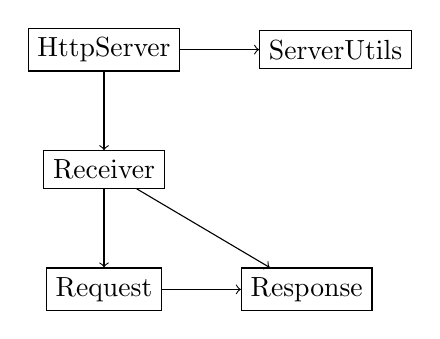
\begin{tikzpicture}
		\node[draw]	(HttpServer) {HttpServer};
		\node[draw, right=of HttpServer]	(ServerUtils) {ServerUtils};
		\node[draw, below=of HttpServer]	(Receiver) {Receiver};
		\node[draw, below=of Receiver]	(Request) {Request};
		\node[draw, right=of Request]	(Response) {Response};
		
		\graph {
			(HttpServer) -> (ServerUtils);
			(HttpServer) -> (Receiver) -> (Request) -> (Response);
			(Receiver) -> (Response);
		};
	\end{tikzpicture}
	\caption{模块关系图} \label{fig1}
\end{figure}
\section{系统实现}

\subsection{HttpServer}

\subsubsection{成员变量}

有成员变量serverSocket,为监听套接字。

\subsubsection{main()方法}

HttpServer.main()方法首先尝试调用ServerUtils.load(),初始化配置。这些配置通过ServerUtils相应Getter访问。

因为本程序没有GUI,所以通过ctrl+c来结束程序,因此需要捕获结束信号。HttpServer.main()接下来通过Runtime.getRuntime().addShutdownHook()来截获ctrl+c信号,当用户试图ctrl+c时,先打印出关闭服务器提示,接下来检查serverSocket的关闭状态,如果没有关闭就关闭它。注册完控制程序以后,打印关闭服务器的提示信息。

注册完关闭程序以后创建监听在ServerUtils中给出的地址的套接字,赋给serverSocket。然后在死循环里试图进行serverSocket.accept(),若无请求到达自然在阻塞状态,若有请求就根据请求的socket创建一个Receiver,新开一个线程执行Receiver.run()。

\vspace*{2\baselineskip} 

这些方法中语句可能出现的异常都用try-catch语句捕捉并打印提示信息。

\subsection{ServerUtils}

\subsubsection{成员变量}

有localIp、port、basePath三个静态变量,分别代表本Web服务器监听的IP、端口号、基路径。不支持热更换配置。

\subsubsection{load()方法}

Web服务器的配置都存放在config.properties中。properties 是Java常用的配置文件,一行一个key=value。

ServerUtils.load()方法首先读取config.properties到localIp、port、basePath三个变量中。读取的过程中对basePath的合法性进行校验,如果其不存在或者是不是目录,校验都不通过。

\vspace*{2\baselineskip} 

这些方法中语句可能出现的异常都用try-catch语句捕捉并打印提示信息。

\subsection{Receiver}

\subsubsection{成员变量}

有成员变量socket,为待处理的请求套接字。

\subsubsection{构造函数}

构造函数接收一个socket,保存到自己的成员变量中。

\subsubsection{run()方法}

考虑到Receiver实现了Runnable接口,故应override Receiver.run()方法。它首先取得socket的inputStream和outputStream,根据inputStream构造Request对象,传入请求 的IP地址和端口号调用Request.parse()方法进行分析;然后根据outputStream构造Response对象,传入分析完毕的Request对象调用Response.constructResponse()以构造返回,最后调用Response.fillResponse()写入响应。

Receiver.run()方法最后调用Receiver.socketClose()来关闭请求套接字。

\subsubsection{socketClose()方法}

Receiver.socketClose()方法检查请求套接字,如果其存在且未被关闭就关闭它。

\vspace*{2\baselineskip} 

这些方法中语句可能出现的异常都用try-catch语句捕捉并打印提示信息。

\subsection{Request}

\subsubsection{成员变量}

inputStream代表请求套接字的读入流,parseSuccess标记着识别请求是否成功,method、uri、httpVerson和HTTP请求对应,分别为请求的方法、URI、协议。

\subsubsection{构造函数}

把传入的读取流保存到成员变量。

\subsubsection{parse()方法}

Request.parse()首先读取读入流的第一行,按空格split成三部分,分别作为method、uri、httpVersion。如果split失败则报告识别错误并返回。特别注意uri要按照UTF-8解码,否则定位本地中文文件名文件会出问题。

按照一定的格式打印出日志头,随即忠实地打印出请求的其他部分(包括请求头)作为日志。

只支持HTTP请求。

\vspace*{2\baselineskip} 

这些方法中语句可能出现的异常都用try-catch语句捕捉并打印提示信息。

\subsection{Response}

\subsubsection{成员变量}

outputStream代表请求套接字的写入流。statusCode是将返回的状态码,会根据这个构造返回。willFile是期待的返回文件。

\subsubsection{构造函数}

把传入的写入流保存到成员变量。

\subsubsection{constructResponse()方法}

Response.constructResponse()方法首先判断请求分析是否成功,不成功或者请求方法不是GET都设置状态码为400,意为bad request。将请求URI正规化以后和基路径拼接再正规化就能够避免路径遍历攻击,从而得到了willFile。

如果willFile是文件夹,根据Web服务器的常见实现,应该尝试返回文件夹下的index.html文件。如果willFile不存在,则设置状态码为404,意为not found。

其他情况状态码为200,即OK。

\subsubsection{fillResponse()}

Response.fillResponse()方法根据状态码来构造不同的返回。如果不是200,就直接返回设计好的报文。如果是200,就先写入一些报文头,计算文件的类型、长度并写入报文,然后将文件写入报文中。

文件类型的计算直接使用Files.probeContentType()方法。

\vspace*{2\baselineskip} 

这些方法中语句可能出现的异常都用try-catch语句捕捉并打印提示信息。

\section{系统测试与结果说明}

配置config.properties和启动以后的结果如图\ref{fig2}所示。
\begin{figure}[htbp]
\centering
\includegraphics[width=0.7\textwidth]{images/1.png}
\caption{配置与启动}
\label{fig2}
\end{figure}

服务器将展示图\ref{fig3}中的内容,这是我的静态个人博客,包括多种类型的文件。

\begin{figure}[htbp]
	\centering
	\includegraphics[width=0.7\textwidth]{images/2.png}
	\caption{服务器的基路径内容}
	\label{fig3}
\end{figure}

打开提供的URL进入主页面如图\ref{fig4}所示。

\begin{figure}[htbp]
	\centering
	\includegraphics[width=0.7\textwidth]{images/3.png}
	\caption{服务器主页面}
	\label{fig4}
\end{figure}

这个过程中,请求和部分响应报文如图\ref{fig5}所示。

\begin{figure}[htbp]
	\centering
	\includegraphics[width=0.7\textwidth]{images/4.png}
	\caption{请求展示与响应报文}
	\label{fig5}
\end{figure}

在服务器侧,可以看到图\ref{fig6}所示的日志。

\begin{figure}[htbp]
	\centering
	\includegraphics[width=0.7\textwidth]{images/5.png}
	\caption{打印请求}
	\label{fig6}
\end{figure}

如图\ref{fig7}所示,可以展示图片。

\begin{figure}[htbp]
	\centering
	\includegraphics[width=0.7\textwidth]{images/6.png}
	\caption{图片显示}
	\label{fig7}
\end{figure}

如\ref{fig8}所示,也支持视频的传输。

\begin{figure}[htbp]
	\centering
	\includegraphics[width=0.7\textwidth]{images/7.png}
	\caption{播放视频}
	\label{fig8}
\end{figure}

试图访问不存在的页面时,会展示404,如\ref{fig9}所示。

\begin{figure}[htbp]
	\centering
	\includegraphics[width=0.7\textwidth]{images/8.png}
	\caption{访问不存在页面}
	\label{fig9}
\end{figure}

如果配置得当,那么在其他的设备上也可以访问网站,如图\ref{fig10}所示。

\begin{figure}[htbp]
	\centering
	\includegraphics[width=0.7\textwidth]{images/9.jpg}
	\caption{其他设备访问}
	\label{fig10}
\end{figure}

\section{改进方向}

\paragraph{线程池} 每收到一个请求,就开一个线程去处理,显然是一种野蛮、粗糙的做法。在请求量大时,合理的做法是开一个线程池,限制可以执行的线程数,同时不至于频繁创建关闭线程。

\paragraph{硬编码} 在代码里硬编码返回报文的一部分也是不好的做法。可以考虑将返回报文的模板保存到特殊的文件夹,根据模板拼接报文。

\paragraph{视频分片} 视频虽然能播放,但是不能随意拖动,只能看已缓冲的部分。将来可以加入对视频分片的支持。

\paragraph{多线程日志混乱} 直接打印到控制台会引发多线程日志混乱打印的问题,应该合理使用日志库。

\section{总结}

本次实验完成了一个Web服务器,总体完成度不错,已经具备良好的可用性。但在大规模请求、多线程部分还有待改善。从这次实验中,我强化了TCP、HTTP的概念,进一步了解了socket编程的步骤,感受到了计算机网络的魅力。
	
\end{document}

